% !TEX root = ../thesis-example.tex
%
\chapter{Analytical Solutions for Barrier Options}

There are closed-form solutions for pricing European-style barrier options. This means we have an explicit mathematical expression that can be used to compute the value of a function without the need for numerical solutions. However, we will continue to compare closed-form solutions to more rigorous methodologies. Unlike their continuous counterparts, no closed-form solutions exist for discrete-time barrier options (even numerical pricing is a challenge). For this reason, we will only focus on continuous-time, single-barrier options.

\section{The Black-Scholes Model}

The Black and Scholes model was first published in 1973, named after the two economist who helped to develop it: Fischer Black and Myrion Scholes. (the model is formally known as the Black-Scholes-Merton model) A rigorous derivation of the Wiener process, Ito's lemma, the portfolio process at the risk-free rate gives us the following equation
\begin{equation}\label{eq:BSM}
	\frac{1}{2}\sigma^2S^2\frac{\partial^2 f}{\partial S^2}+rS\frac{\partial f}{\partial S}-\frac{\partial f}{\partial }-rf=0
\end{equation}
From here, we solve equation (\ref{eq:BSM}) to arrive at the following equation
\begin{equation}\label{eq:bs_call_option}
	f(S,t)=Se^{-qT}N(d_1)-Ke^{-rT}N(d_2)
\end{equation}
where $S$ is the stock price, $K$ is the strike price, $r$ is the risk-free rate, $T$ is the time to expiration, $\sigma$ is the volatility of the stock, $N(\cdot)$ is the cumulative distribution function, and $d_1/d_2$ are derived by the following:
\begin{equation}
	d_1=\frac{\ln\left(\sfrac{S_0}{K}\right)+\left(r+\sfrac{\sigma^2}{2}\right)T}{\sigma\sqrt{T}},\quad d_2=\frac{\ln\left(\sfrac{S_0}{K}\right)+\left(r-\sfrac{\sigma^2}{2}\right)T}{\sigma\sqrt{T}}=d_1-\sigma\sqrt{T}
\end{equation}
A more rigourous proof for the solution to the Black-Scholes PDE can be found on \ref{section:A1} of the appendix.
\section{Analytical Solution to Barrier Options}

We start by changing the value of $T$ for $\tau=T-t$. From there, in order to have the PDE solutioni for the up-and-out call option, we begin to alter equation (\ref{eq:bs_call_option}). Let $H$ be the barrier price. Then when $B\geq K$, we have:
\begin{equation}\label{eq:DOC}
	C_{\text{up-out}}(S,t)=Se^{-q\tau}\left(N(d_1)-\left(\frac{B}{S}\right)^{2\lambda}N(d^\prime_1)\right)-Ke^{-r\tau}\left(N(d_2)-\left(\frac{B}{S}\right)^{2\lambda-2} N(d^\prime_2)\right)
\end{equation}
where
\begin{equation}
	\lambda=\frac{r-q}{\sigma^2}+\frac{1}{2}
\end{equation}
and $d^\prime_1/d^\prime_2$ is derived by the following
\begin{equation}
	d^\prime_1=\frac{\ln\left(\frac{B^2}{SK}\right)+(r-q+\tfrac{1}{2}\sigma^2)\tau}{\sigma\sqrt{T}},\quad d^\prime_2=d^\prime_1-\sigma\sqrt{\tau}
\end{equation}
If $S\geq B$ at any time before expiration, the up-and-out call ceases to exist (it is knocked out). If $S<B$ for the entire option's life, the payoff at maturity is just like a standard call, where the payoff is $\max\left(S_T-K, 0\right)$
\section{Barrier Call/Put Parity}

An interesting consequence from the analytical solution to barrier options is the relationship between knock-in and knock-out barrier options. As such, in the same way there is a parity relationship between vanilla puts and calls, there is a parity relationship between knock-out calls/puts and knock-in calls/puts. We refer to this relationship as the up-out/up-in call/put parity. For this example, we will refer to the up-in and up-out call option.

The parity between the up-in and up-out call option demonstrates that the price of an up-and-in call option can be expressed by the following:

\begin{equation}
	C_{\text{vanilla}}=C_{\text{up-in}}+C_{\text{up-out}}
\end{equation}
This parity holds under the assumption that no dividends are paid, and other assumptions like interest rates are constant. This relationship works because the vanilla call represents a basic option that can be exercised at 

\section{Barrier Option Payoffs}

With eight different types of single barrier options comes eight possible payoffs, based on the barrier price. Table (\ref{tab:barrier_payoff}) shows the payoff based on whether the barrier is up or down, whether the stock price in or outside of the barrier, and whether the option type is a call or put. Refer to Appendix \ref{section:A2}

\begin{table}[htbp!]
	\centering
	\begin{tabular}{|c|c|c|c|c|}
		\hline
		Down/Up & In/Out & Call/Put & Payoff ($K\leq B$) & Payoff ($K\geq B$)  \\
		\hline
		Down   & In     & Call      & $A_1-A_2+A_4+A_5$     & $A_3+A_5$   \\
		 \hline
		Up   & In     & Call      & $A_2-A_2+A_4+A_5$     & $A_1+A_5$   \\
		 \hline
		Down   & In     & Put    &  $A_1+A_5$  & $A_2-A_3+A_4+A_5$   \\
		\hline
		Up   & In     & Put    &  $A_3+A_5$  & $A_1-A_2+A_4+A_5$  \\
		\hline		
		Down   & Out     & Call    &  $A_2-A_4+A_6$  & $A_1-A_3+A_6$  \\
		\hline
		Up   & Out     & Call    &  $A_1-A_2+A_3-A_4+A_6$  & $A_6$  \\
		\hline
		Down   & Out     & Put    &  $A_6$  & $A_1-A_2+A_3-A_4+A_6$  \\
		\hline
		Up   & Out     & Put    &  $A_1-A_3+A_6$  & $A_2-A_4+A_6$  \\
		\hline
	\end{tabular}
	\label{tab:barrier_payoff}
	\caption{Theoretical Values of Single Barrier Options}
\end{table}
Throughout this report, we will be deriving our analysis from the up-and-out call and put option, since it is easier to intuitively understand. The payoffs from equations (\ref{eq:vanilla_call}) and (\ref{eq:vanilla_put}), still hold for vanilla calls and puts. However, recall for a knocked-out up option, the option losses value once it has reaches the barrier above the underlying stock price.

\section{Surface of the Barrier Option}

\begin{figure}[H]
	\centering
	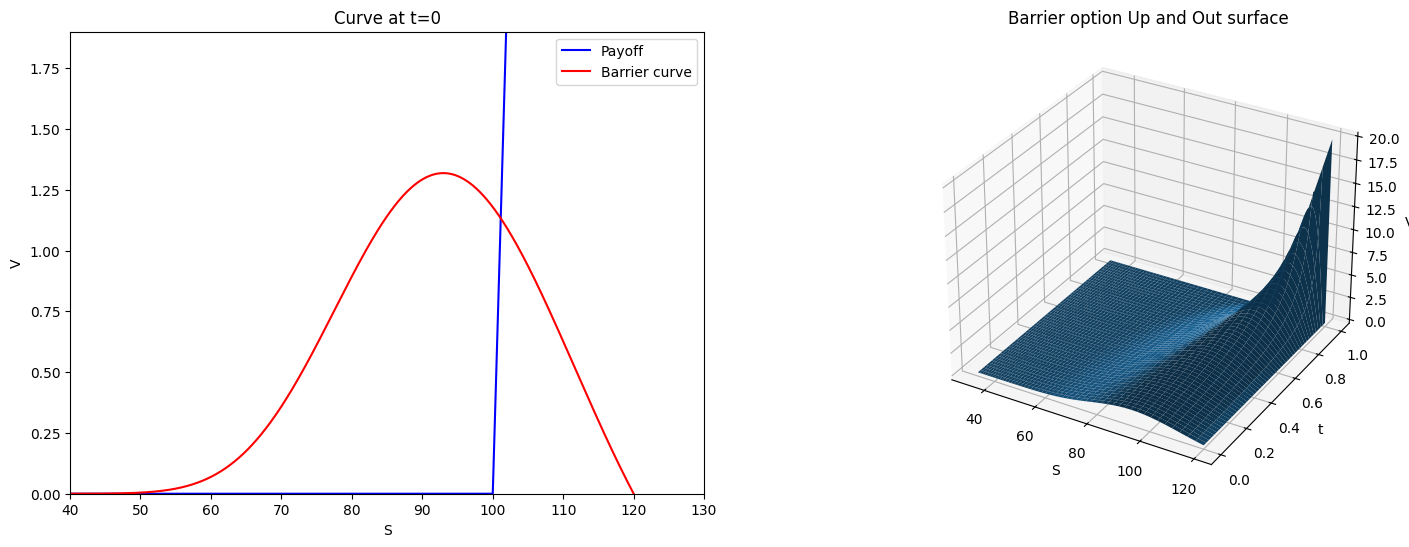
\includegraphics[width=.90\linewidth]{content/images/surface.png}
	\caption{At-the-money up-and-out barrier option}
	\label{fig:surface}
\end{figure}

Figure (\ref{fig:surface}) shows the barrier curve and surface for an at-the-money up-and-out barrier option for $S=100,K=100, T=1, r=10\%,\sigma=20\%, \text{ and }B=120$. The curve assumes the option is close to or at expiration date. As we can see, the option has no value at any price below 100, as the strike price is also 100. However, the call will retain some value, as the option has not reached the barrier of 120. Where the payoff line (blue) and the barrier curve (red) intersects shows the potential payoff at expiration, which is 1.18 according to Black-Scholes.

The surface shows the option value in relation to time and the underlying price. As we can see, the barrier option has the most value when the option is very close to expiration and the stock price is relatively close to the barrier. Otherwise, the option has no value when the underlying is at 40 and the time to expiration is 0. The option also loses it's value when the option is close to the barrier.
